\documentclass[xcolor={usenames,dvipsnames}]{beamer}
%\documentclass[draft]{beamer}


\usepackage[dvipsnames]{xcolor}



\usepackage[utf8]{inputenc}
\usepackage[T1]{fontenc}
\usetheme{MOKAbeamer}

%\usepackage[french]{babel}



\usepackage{tikz}

%\usepackage[draft]{animate}
\usepackage{animate}
\usepackage{ifthen}
\usepackage{filecontents}
\usepackage{stmaryrd}
\usepackage{listliketab}

\usepackage{multirow}

\usetikzlibrary{calc}
\usepackage{pifont}
\usepackage{mystyle}

\usepackage{tabularx}

\usepackage{algorithm,algorithmic}

\usepackage{standalone} % pour compiler les tikz -> input
\definecolor{vertsombre}{rgb}{0.0,0.5,0.0}
\usepackage{array}
\newcolumntype{M}{>{\centering\arraybackslash} m{0.5cm} }

\newcommand{\cyte}[1]{{\scriptsize\color{domcolor}#1}}
\newcommand{\cyteb}[1]{{\footnotesize\color{white}#1}}

%Pour ne pas compter les derniers slides
\newcommand{\backupbegin}{
   \newcounter{finalframe}
   \setcounter{finalframe}{\value{framenumber}}
}
\newcommand{\backupend}{
   \setcounter{framenumber}{\value{finalframe}}
}


%\newtheorem{theorem}{Theorem}[chapter]
%\newtheorem{lemma}[theorem]{Lemma}
\newtheorem{prop}[theorem]{Proposition}
%\newtheorem{corollary}[theorem]{Corollary}
%\newtheorem{definition}[theorem]{Definition \rm}
%\newtheorem{definition}[theorem]{Definition}
\newtheorem{remark}[theorem]{Remark}

%Debug boxes
\showboxdepth=5
\showboxbreadth=5


\newcommand{\nfb}[1]{\begin{frame}[allowframebreaks]#1\end{frame}}





\BeforeBeginEnvironment{definition}{%
    \setbeamercolor{block title}{fg=white,bg=thirdcolor!60!white!}
    \setbeamercolor{block body}{fg=black,bg=lightthird}
}
\AfterEndEnvironment{definition}{
        \setbeamercolor{block title}{fg=white,bg=domcolor}
        \setbeamercolor{block body}{fg=black,bg=lightdom}
}


%\graphicspath{{/Users/claireboyer/Documents/Enseignement/MachineLearning/ISUP2019/slides/cours1/}{/Users/claireboyer/Documents/Enseignement/MachineLearning/ISUP2019/slides/cours3/}{/Users/claireboyer/Documents/Enseignement/MachineLearning/ISUP2018/slides/cours1/}{/Users/claireboyer/Documents/Enseignement/MachineLearning/ISUP2018/}}

\begin{document}
\title[]{Gradient based optimization}
\author[S.~Le Corff]{Sylvain Le Corff}
\date{}

\begin{frame}[plain]
\titlepage
\end{frame}


\section{Motivation in Machine Learning}

\subsection{Logistic regression}

\begin{frame}{Semi-parametric modelling - logistic regression}


$\rightharpoondown$ The objective is to \alert{predict the  label $Y\in\{0,1\}$} based on $X\in\mathbb{R}^d$.

$\rightharpoondown$ Logistic regression \alert{models the distribution of $Y$ given $X$}.

\vspace{-.2cm}

%{\bf\textcolor{violet}{The model}} 
\begin{equation*}
\P(Y = 1| X) = \sigma(\langle w,X \rangle + b)\,,
\end{equation*}

where $w \in \R^d$ is a vector of model \textbf{weights} and $b \in \R$ is the \textbf{intercept}, and where $\sigma$ is the \textbf{sigmoid} function.

\vspace{.3cm}
 
\begin{tabular}{cc}
	\begin{minipage}{0.4\textwidth}
		\begin{equation*}
		\sigma: z \mapsto \frac{1}{1 + e^{-z}}\,.
		\end{equation*}%    
	\end{minipage}
	&
	\begin{minipage}{0.4\textwidth}
		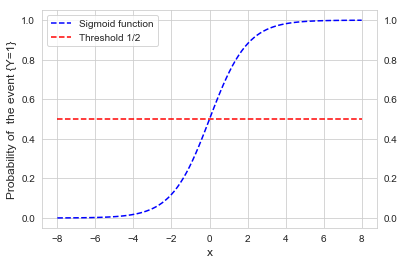
\includegraphics[width=5cm]{./sigmoid.png}  
	\end{minipage}    
\end{tabular}

$\rightharpoondown$ The sigmoid function is a \alert{model choice to map $\mathbb{R}$ into $(0,1)$}.

$\rightharpoondown$ Another widespread solution for $\sigma$ is $\sigma: z \mapsto  \P( Z \leqslant z)$ where $Z\sim \mathcal{N}(0,1)$, which leads to a \textbf{probit} regression model.

\end{frame}



\begin{frame}{Logistic regression}

{\bf\textcolor{violet}{Log-odd ratio}}

\begin{align*}
\Acolorboxed{&
\log \Big( \P(Y=1 | X)\Big) - \log \Big(\P(Y = 0| X) \Big) 
= \langle w,X \rangle  + b\,.}
\end{align*}

\vspace{.3cm}

{\bf\textcolor{violet}{Classification rule}}

 Note that 
\begin{equation*}
\P(Y = 1| X) \geq \P(Y = 0| X)
\end{equation*}
if and only if
\begin{equation*}
\langle w,x \rangle + b \geqslant 0\,.
\end{equation*}

$\rightharpoondown$ This is a \textbf{\alert{linear classification}} rule.

$\rightharpoondown$ This classifier requires to \alert{estimate $w$ and $b$}.

\end{frame}

\begin{frame}{Logistic regression}

$\rightharpoondown$   $\{(X_i,Y_i)\}_{1\leqslant i\leqslant n}$ are \alert{i.i.d. with the same distribution as $(X,Y)$}.

{\bf\textcolor{violet}{Likelihood}}

\begin{align*}
 \prod_{i=1}^n \P(Y_i | X_i) &= \prod_{i=1}^n \sigma(\langle w,X_i \rangle + b)^{Y_i} \big(1 - 
\sigma(\langle w,X_i \rangle + b) \big)^{1 - Y_i}\,, \\
& = \prod_{i=1}^n \sigma(\langle w,x_i \rangle + b)^{Y_i} 
\sigma(-\langle w,X_i \rangle - b)^{1 - Y_i}
\end{align*}
\smallskip

and the \alert{normalized negative loglikelihood} is 
\smallskip

\begin{equation*}
f(w,b) = \frac{1}{n}\sum_{i=1}^n \ell(Y_i, \langle w,X_i \rangle + b)\,.
\end{equation*}
\end{frame}


\begin{frame}{Logistic regression}
		
Compute $\hat w_n$ and $\hat b_n$ as follows:

\begin{align*}
\Acolorboxed{&
(\hat w_n, \hat b_n) \in \argmin_{w \in \R^d, b \in \R}
\frac 1n \sum_{i=1}^n\left(-Y_i (X_i^T w+ b) +  \log(1+ e^{X_i^Tw + b})\right)\,.}
\end{align*}

\vspace{.3cm}

$\rightharpoondown$ It is an \textbf{average of losses}, one for each sample point.

$\rightharpoondown$ It is a \alert{convex and smooth problem}.


\medskip

Using the \textbf{\alert{logistic loss}} function
\smallskip 

\begin{equation*}
\ell: (y, y') \mapsto \log(1 + e^{-y y'}) 
\end{equation*}

yields

\begin{equation*}
(\hat w_n, \hat b_n) \in \argmin_{w \in \R^d, b \in \R}
\frac 1n \sum_{i=1}^n \ell(Y_i, \langle w,X_i \rangle + b)\,.
\end{equation*}
\end{frame}


\begin{frame}{Maximum likelihood estimate}
Assume for now that the intercept is 0. Then, the likelihood is,

$$
L_n(w)  =  \prod_{i=1}^n \left(\frac{e^{X_i^Tw}}{1+e^{X_i^T w}} \right)^{Y_i} \left(\frac{1}{1+e^{X_i^T w}} \right)^{1-Y_i} = \prod_{i=1}^n \left(\frac{e^{X_i^Tw Y_i}}{1+e^{X_i^T w}} \right)\,.
$$

And the \alert{negative $\log$-likelihood} is

\begin{align*}
\ell_n(w) = - \log(L_n(w)) =  \sum_{i=1}^n \left(-Y_i X_i^T w+ \log(1+ e^{X_i^Tw})\right)\,.
\end{align*}

{\bf\textcolor{violet}{Derivatives}}

%$$
%\nabla  \left(\log(L_n(\beta))\right)=   \left(\frac{\partial}{\partial \beta_0}(\beta),\cdots, \frac{\partial}{\partial \beta_d}(\beta)\right)\,. 
%$$

\begin{eqnarray*}
\frac{\partial \left(\log(L_n(w))\right)}{\partial w_j}&= &
\sum_{i=1}^n \left(Y_i X_{ij}
	- \frac{x_{ij} e^{X_i^T
	w}}{(1+ e^{X_i^T
	w})}   \right) \\
&=& \sum_{i=1}^n X_{ij} \left(Y_i - \sigma(\langle w,X_i \rangle)\right)\,.
\end{eqnarray*}

$\rightharpoondown$ \alert{No explicit solution} for the maximizer of the loglikelihood... Parameter estimate obtained using \alert{gradient based optimization}.

\end{frame}


\subsection{Feed forward neural networks}

\begin{frame}{Feed Forward Network}

\begin{center}
\includegraphics[width = 0.75\textwidth]{ffnn4.png}
\end{center}

$\rightharpoondown$ $X$ \alert{input in $\R^d$}.

$\rightharpoondown$ $z^h(X)$ \alert{pre-activation in $\R^H$}, with \alert{weight $W^h\in\R^{dxH}$} and \alert{bias $b^h\in\R^H$}.

$\rightharpoondown$ $g$ \alert{any activation function} to produce $h\in\R^H$.

$\rightharpoondown$ $z^o(X)$ \alert{pre-activation in $\R^M$}, with \alert{weight $W^o\in\R^{HxM}$} and \alert{bias $b^o\in\R^M$}.

$\rightharpoondown$  Apply the \alert{softmax function to produce the output}, i.e. $\mathbb{P}(Y=m|X)$ for $1\leqslant m \leqslant M$.
\end{frame}

%\subsection{Support Vector Machine}
%
%
%\begin{frame}
%\frametitle{Support Vector Machine}
%
%A dataset is \textbf{\textcolor{violet}{linearly separable}} if there exists an hyperplane $H_{w,b}$ such that: 
%\medskip
%
%$\rightharpoondown$ Points $x_i \in \R^d$ such that \alert{$Y_i = 1$ on one side of the hyperplane}.
%
%$\rightharpoondown$ Points $x_i \in \R^d$ such that \alert{$Y_i = -1$ on the other}.
%
%$\rightharpoondown$ $H_{w,b}$ \alert{does not pass through any point $X_i$}.
%
%
%\bigskip
%
%\begin{columns}[T] % align columns
%	\begin{column}{.5\textwidth}
%		\begin{center}
%			\includegraphics[width=0.65\textwidth]{./hyperplane.png}
%		\end{center}
%		
%	\end{column}%
%	\hspace{-0.2cm}
%	\begin{column}{.5\textwidth}
%		
%		An hyperplane 
%		
%		\smallskip
%		\begin{equation*}
%			H_{w,b} = \{ x \in \R^d : \inr{w, x} + b = 0 \}\,.
%		\end{equation*}
%	\smallskip
%	
%		is a translation of a set of vectors orthogonal to $w$.
%		
%	\end{column}%
%\end{columns}
%
%
%
%\end{frame}
%
%
%
%
%\begin{frame}
%	\frametitle{Support Vector Machine}
%	
%	
%	
%$H_{w,b}$ is \alert{invariant by multiplication of $w$ and $b$ by a nonzero scalar}.
%
%\bigskip
%
%If $H_{w,b}$ does not pass through any sample point $X_i$,  $w$ and $b$ can be scaled so that
%
%\smallskip 
%
%\begin{equation*}
%\min_{(X_i, Y_i)_{1\leqslant i\leqslant n}} |\inr{w, X_i} + b| = 1\,.
%\end{equation*}
%\begin{center}
%\includegraphics[width=0.5\textwidth]{./canonical_hyperplane.png}
%\end{center}
%
%For such $w$ and $b$, $H_{w,b}$ is said to be the \alert{\emph{canonical} hyperplane}.
%\end{frame}
%
%
%\begin{frame}[t]\frametitle{Support Vector Machine}
%	
%	
%	
%The \alert{distance of any point $z \in \R^d$ to $H_{w,b}$} is 
%
%\smallskip 
%
%\begin{equation*}
%d(z,H_{w,b}) = \frac{|\inr{w, x'} + b|}{\norm{w}}\,.
%\end{equation*}
%
%
%\begin{center}
%\includegraphics[width=3.8cm]{./margin.jpg}
%\end{center}
%		
%
%
%If $H_{w,b}$ is a canonical hyperplane, its \alert{\textbf{margin}} is 
%
%	
%\begin{equation*}
%\max_{(X_i, Y_i)_{1\leqslant i\leqslant n}}   \frac{|\inr{w, X_i} + b|}{\norm{w}} = \frac{1}{\norm{w}}\,.
%\end{equation*}
%
%\end{frame}
%
%
%\begin{frame}
%	\frametitle{Support Vector Machine}
%	
%
%If the \alert{dataset is strictly linearly separable}, there exists a canonical separating hyperplane 
%
%\smallskip
%\begin{equation*}
%H_{w,b} = \{ x \in \R^d : \inr{w, x} + b = 0 \}\,,
%\end{equation*}
%\smallskip
%
%that satisfies, for any $1\leqslant i\leqslant n$,
%\smallskip
%\begin{equation*}
%|\inr{w, x_i} + b| \geqslant 1\,,
%\end{equation*}
%\smallskip
%
%which entails that a point $X_i$ is correctly classified if
%
%\smallskip
%\begin{equation*}
%Y_i (\langle w,X_i \rangle + b) \geqslant 1.
%\end{equation*}
%
%\medskip
%
%The \alert{margin of $H_{w,b}$ is equal to $1 / \norm{w}$}.
%\end{frame}
%
%
%
%\begin{frame}
%	\frametitle{Support Vector Machine}
%	
%	
%
%\textbf{\textcolor{violet}{Linear SVM: separable case}}
%
%\bigskip
%
%A classifier \alert{with maximum margin} can be obtained by solving the following problem:
%\begin{align*}
%\min_{w \in \R^d, b \in \R} \frac 12 \norm{w}_2^2\,,
%\end{align*}
%under the \alert{constraints $Y_i (\langle w,X_i \rangle + b) \geqslant 1$ for all $1\leqslant i\leqslant n$}.
%
%
%\bigskip
%
%$\rightharpoondown$ This problem admits a \textbf{unique} solution.
%
%$\rightharpoondown$ It is a \textcolor{violet}{quadratic programming' problem}, which is easy to solve numerically.
%
%$\rightharpoondown$ \textcolor{violet}{Dedicated optimization algorithms can solve this on a large scale} very efficiently.
%
%\end{frame}
%
%\begin{frame}
%	\frametitle{SVM for the non linearly separable case}
%	
%$\rightharpoondown$ \textbf{\textcolor{violet}{Introduce slack variables $\xi_i \geqslant 0$ to model errors}}.
%	
%
%		
%		$
%		\begin{cases}
%		\textrm{\alert{no error}}~ & Y_i (\langle w , X_i \rangle + b ) \geqslant 1 \Rightarrow \xi_i = 0\\
%		\textrm{\alert{error}}~ & Y_i (\langle w , X_i \rangle + b ) < 1 \Rightarrow \xi_i = 1 - Y_i (\langle w , X_i \rangle + b ) > 0\,.\\
%		\end{cases}
%		$
%
%
%
%	
%	\begin{center}
%		\includegraphics[scale=0.4]{./SVM-with-soft-margin-kernel-with-different-cases-of-slack-variables.jpg}
%	\end{center}
%	
%\end{frame}
%
%\begin{frame}\frametitle{New optimization problem}
%
%Compute $\hat w_n$ and $\hat b_n$ as follows:
%
%\begin{align*}
%\Acolorboxed{&
%\min_{w, b , \xi} \frac 12 \norm{w}_2^2 + C \sum_{i=1}^n \xi_i\,,}
%\end{align*}
%
%\vspace{.2cm}
%
%under the constraints, $Y_i (\langle w,X_i \rangle+ b) \geqslant 1 - \xi_i$ and $\xi_i \geqslant 0$ for all $1\leqslant i\leqslant n$.
%	
%
%\bigskip
%
%\alert{Introducing the hinge loss $\ell:(y,y') \mapsto \max(0, 1- yy')$}, the optimization can be rewritten as
%
%\medskip
%
%\textbf{\textcolor{violet}{SVM with hinge loss}}
%
%\begin{align*}
%\Acolorboxed{&
%\min_{w, b} \frac 12 \norm{w}_2^2 + C \sum_{i=1}^n \ell(y_i, \hat{y}_i)\,.}
%\end{align*}
%	
%\end{frame}



\subsection{General formulation}

\begin{frame}
	\frametitle{General optimization problem}
	
\alert{Parameter inference in machine learning} often boils down to solving

\begin{equation*}
\argmin_{w \in \R^d} f(w) + g(w)\,,
\end{equation*}

with $f$ a \alert{goodness-of-fit functio  based on a loss $\ell$},

\begin{equation*}
f(w) = \frac 1n \sum_{i=1}^n \ell(y_i, \langle w, x_i \rangle)
\end{equation*}

 and

\begin{equation*}
g(w) = \lambda \pen(w)\,,
\end{equation*}

where $\lambda>0$ and \alert{$\pen(\cdot)$ is some penalization function}.

%Examples of penalization functions:

$\rightharpoondown$ \textcolor{violet}{$\pen(w) =  \|w\|_2^2$ (Ridge).}

$\rightharpoondown$ \textcolor{violet}{$\pen(w) = \|w\|_1$ (Lasso)}.


\end{frame}




%\begin{frame}
%\frametitle{Different losses for classification}
%
%\alert{Logistic loss}, $\ell(y, y') = \log(1 + e^{-y y'})$.
%
%\vspace{.2cm}
%
%\alert{Hinge loss}, $\ell(y, y') = (1 - y y')_+$.
%
%\vspace{.2cm}
%
%\alert{Quadratic hinge loss},  $\ell(y, y') = \frac 12 (1 - y y')_+^2$.
%
%\vspace{.2cm}
%
%\alert{Huber loss} $\ell(y, y') = -4 y y' \mathds{1}_{y y' < -1} + (1 - y y')_+^2 \mathds{1}_{y y' \geq -1}$.
%
%\begin{center}
%\includegraphics[width=0.65\textheight]{./losses_classif.png}
%\end{center}
%
%$\rightharpoondown$  These losses can be understood as a \textcolor{violet}{convex approximations of the 0/1 loss $\ell(y, y') = \mathds{1}_{y y' \leq 0}$}.
%
%\end{frame}





\section{Gradient descent procedures}

\subsection{Gradient Descent}

%\begin{frame}
%	\frametitle{Minimization problems}
%	
%	\begin{center}
%		{\LARGE
%			Aim: minimizing a function $h: \R^d \to \R$
%			
%			\vspace{0.5cm}
%			
%			$d$: dimension of the search space.
%		}
%	\end{center}
%	
%	\vspace{0.5cm}
%	
%	\begin{center}
%		\includegraphics[scale=0.6]{./global_local_minima}
%	\end{center}
%	
%\end{frame}
%
%
%\begin{frame}
%	\frametitle{Level sets}
%	
%	One-dimensional (1-D) representations are often misleading, we therefore often represent level-sets of
%	functions
%	
%	$$
%	\mathcal{C}_c = \{ \bx \in \R^d, f(\bx) = c\}.
%	$$
%	
%	\vspace{0.3cm}
%	
%	{\bf Example of level sets in dimension two}
%	
%	\begin{center}
%		\includegraphics[scale=0.6]{./2d_level_sets}
%	\end{center}
%\end{frame}
%
%
%

\begin{frame}
	\frametitle{Exhaustive search}
	
	
\begin{align*}
\Acolorboxed{&
w^{\star} \in \argmin_{w \in [0,1]^d} f(w)\,.}
\end{align*}

\smallskip

Optimizing on a grid of $[0,1]^d$, when $f$ is regular enough, \alert{requires $\lfloor 1/\varepsilon \rfloor^d$ evaluations  to achieve a precision of order  $\varepsilon$}. 

Evaluating the expression
$$
f: x \mapsto \sum_{i=1}^d x_i^2,
$$
to obtain a precision of $\varepsilon = 10^{-2}$ requires  \alert{$1,75. 10^{-3}$ seconds in dimension $1$ and $1,75. 10^{15}$ seconds in dimension $10$}, i.e., nearly 32 millions years. 

\vspace{.3cm}

$\rightharpoondown$  Prohibitive in high dimensions (curse of dimensionality).
\end{frame}


\begin{frame}{First order necessary condition}
	
$\rightharpoondown$ {\bf \textcolor{violet}{In dimension one}}.
		
Let $f : \R \to \R$ be a differentiable function. If $x^{\star}$ is a local extremum (minimum/maximum) then $f'(x^{\star}) = 0$.
		
\begin{center}
\includegraphics[scale=0.6]{./extrema_f}
\end{center}
	
$\rightharpoondown$ {\bf \textcolor{violet}{Generalization for $d>1$}}. 
		
Let $f: \R^d \to \R$ be a differentiable function. If $x^{\star}$ is a local extremum then $\nabla f(x^{\star}) = 0$.
		
\vspace{.6cm}

Points such that $\nabla f(x^{\star}) = 0$ are called \alert{critical points}. 
	
\vspace{.2cm}

\alert{Critical points are not always extrema} (consider $x \mapsto x^3$).	
\end{frame}

\begin{frame}{Gradient}
	
The gradient of a function $f: \R^d \to \R$ in $x\in\R^d$, denoted by $\nabla f (x)$, is \alert{the vector of partial derivatives}:
\begin{align*}
\nabla f(x) =  \begin{pmatrix}
			\frac{\partial f}{\partial x_1} \\
			\vdots \\
			\frac{\partial f}{\partial x_d}
		 \end{pmatrix}\,.
\end{align*}

\textbf{\textcolor{violet}{Some useful gradients}}

$\rightharpoondown$ If $f: \R \to \R$, $\nabla f(x) = f'(x)$.

$\rightharpoondown$ $f:x \mapsto \langle a,x\rangle$: $\nabla f(x) = a$.
	
$\rightharpoondown$ $f:x \mapsto x^T A x$: $\nabla f(x) = (A + A^T) x$.
	
$\rightharpoondown$ Particular case: $f: x \mapsto \|x\|^2$, $\nabla f(x) = 2x$.

\end{frame}


\begin{frame}{Heuristic: why gradient descent works?}
	
For a function $f: \R^d \to \R$, define the \alert{level sets}: 
$$
\mathcal{C}_c = \{ \bx \in \R^d, f(\bx) = c\}\,.
$$
	
	
\begin{center}
\begin{figure}
\includegraphics[scale=0.4]{./gradient_descent_iterations.png}
\caption{Gradient descent for function $f: (x,y) \mapsto x^2 + 2 y^2$}
\end{figure}
\end{center}
	
$\rightharpoondown$  The gradient is \alert{orthogonal to level sets}. 

\end{frame}



\begin{frame}{Convexity}

\textbf{\textcolor{violet}{Convexity - Definition}}

A function $f : \R^d \to \R$ is \alert{convex} on $\R^d$ if, for all $x, y \in \R^d$, for all $\lambda \in [0,1]$,
$$
f(\lambda x + (1- \lambda) y ) \leq \lambda f(x) + (1 - \lambda) f(y).
$$	

\textbf{\textcolor{violet}{Convexity - First derivative}}
		
A \alert{differentiable function $f : \R^d \to \R$} is convex if and only if, for all $x,y\in\R^d$,

\begin{align*}
f(x) \geqslant f(y) + \langle \nabla f (y), x-y \rangle\,. 
\end{align*}
	
\vspace{0.4cm}
	
\begin{center}
\includegraphics[scale=0.5]{./picture_convexity2}
\end{center}
\end{frame}

\begin{frame}
	\frametitle{Hessian}
	
	\large 
	
	If $f: \R^d \to \R$ is \alert{twice differentiable}, the \alert{Hessian matrix in $x\in\R^d$} denoted by $\nabla^2 f(x)$ is given by
	
	\bigskip 

	
\begin{align*}
	\nabla^2 f (x) = 
	\begin{pmatrix}
	\frac{\partial^2 f}{\partial x_1^2}(x) & \frac{\partial^2 f}{\partial x_1 \partial x_2}(x) & \hdots & \frac{\partial^2 f}{\partial x_1 \partial x_d}(x) \\
	\frac{\partial^2 f}{\partial x_2 \partial x_1}(x) & \frac{\partial^2 f}{\partial x_2^2}(x) & \hdots & \frac{\partial^2 f}{\partial x_2 \partial x_d}(x) \\
	\vdots & \vdots & \vdots & \vdots \\
	\frac{\partial^2 f}{\partial x_d \partial x_1}(x) & \frac{\partial^2 f}{\partial x_d \partial x_2}(x) & \hdots & \frac{\partial^2 f}{\partial x_d^2}(x) \\
	\end{pmatrix}\,.
\end{align*}

\bigskip 
	\bigskip 

The \textbf{\textcolor{violet}{Hessian matrix is symmetric if $f$ is twice continuously differentiable}}.

\end{frame}

\begin{frame}
	\frametitle{Convexity}
	
\textbf{\textcolor{violet}{Convexity - Hessian}}

A \alert{twice differentiable function $f : \R^d \to \R$} is convex if and only if, for all $x\in\R^d$,

\begin{align*}
\nabla^2 f(x) \succeq 0\,, 
\end{align*}

that is $h^T \nabla^2 f(x) h \geqslant 0$, for all $h \in \R^d$.

\vspace{0.4cm}

	\begin{center}
		\includegraphics[scale=0.6]{./picture_convexity3}
	\end{center}
\end{frame}





\begin{frame}
	\frametitle{Optimality conditions: second order}
	
	\large
	
	Assume that $f$ is twice continuously differentiable.
	
	\bigskip
	
\textbf{\textcolor{violet}{Necessary condition}}
	
	\bigskip 
	
	If $x^{\star}$ is a local minimum, then \alert{$\nabla f(x^{\star}) = 0$ and $\nabla^2 f(x^{\star})$ is positive semi-definite}. 
	
	\bigskip
	
	\bigskip
	
\textbf{\textcolor{violet}{Sufficient condition}}
	
	\bigskip 
	
	If \alert{$\nabla f(x^{\star}) = 0$ and $\nabla^2 f(x^{\star})$ is positive definite} then $x^{\star}$ is a strict local optimum. 
	
		\bigskip
	

 For $d=1$, this condition boils down to \alert{$f'(x^{\star}) = 0$ and $f''(x^{\star}) >0$}. 
	
\end{frame}



\begin{frame}{Classes of algorithms}
	
	\large 
	
Gradient descent algorithms are  \alert{iterative procedures}. There are two classes of such algorithms, depending on the information that is used to compute the next iteration. 
	
	\bigskip 
	\bigskip
	
\textbf{\textcolor{violet}{First-order algorithms}} that use $f$ and $\nabla f$. Standard algorithms when $f$ is differentiable and convex. 
	
	\bigskip 
	\bigskip
	
\textbf{\textcolor{violet}{Second-order algorithms}} that use $f$, $\nabla f$ and $\nabla^2f$. They are useful when computing the Hessian matrix is not too costly. 
	
	
\end{frame}












\begin{frame}{Gradient descent algorithm}
	


\textbf{\textcolor{violet}{Gradient descent}}
		
\alert{Input}: Function $f$ to minimize, initial vector $w^{(0)}$, $k=0$.

\medskip 
	
	
\alert{Parameters}: step size $\eta>0$.

\medskip
	
While \textit{not converge} do


\hspace{2cm} $\rightharpoondown$ $w^{(k+1)} = w^{(k)} - \eta_{k+1} \nabla f(w^{(k)})$.

\hspace{2cm} $\rightharpoondown$ $k = k+1$.

\medskip

\alert{Output}: $w^{(n_*)}$ where $n_*$ is the last iteration.

	
\end{frame}




\begin{frame}
	\frametitle{When does gradient descent converge?}
	
\textbf{\textcolor{violet}{Convex function}}

A function $f : \R^d \to \R$ is \alert{convex} on $\R^d$ if, for all $x, y \in \R^d$, for all $\lambda \in [0,1]$,
$$
f(\lambda x + (1- \lambda) y ) \leq \lambda f(x) + (1 - \lambda) f(y).
$$	
	

\vspace{.4cm}
	
\textbf{\textcolor{violet}{$L$-smooth function}}

A function $f$ is said to be \alert{$L$-smooth} if $f$ is differentiable and if, for all $x, y \in \R^d$, 
$$
\| \nabla f(x) - \nabla f(y) \| \leqslant L \|x-y\|\,.
$$
	
If $f$ is \alert{twice differentiable}, this is equivalent to writing that for all $x \in \R^d$,  
	
$$
\lambda_{max} (\nabla^2 f(x)) \leqslant L.
$$
	
\end{frame}


\ifinclude{
\begin{frame}[allowframebreaks]
	\frametitle{Proof}
	\begin{block}{Proposition}
		If $f$ is twice differentiable, $f$ is \blue{$L$-smooth} if and only if for all $x \in \R^d$,  $$\lambda_{max} (\nabla^2 f(x)) \leq L.$$
	\end{block}
	
	\blue{Proof}
	\medskip
	
	Fix $x, y \in \R^d$ and $c>0$. Let $g(t) = \nabla f (x + tcy)$. Thus, $g'(t) = [\nabla^2 f(x+tcy)](cy)$. By the mean value theorem, there exists some constant $t_c \in [0,1]$ such that
	
	\begin{align}
	\nabla f (x+cy) - \nabla f(x) = g(1) - g(0) = g'(t_c) = [\nabla^2 f(x+t_c c y )](cy). \label{eq_hessian_gradient}
	\end{align}
	
	\medskip
	\blue{First implication}
	\medskip
	
	Taking the norm of both sides of (\ref{eq_hessian_gradient}) and applying the smoothness condition, we obtain
	
	$$
	\|[\nabla^2 f(x+t_c c y)] y \| \leq L \|y\|.
	$$
	
	By taking $c \to 0$ and using the fact that $t_c \in [0,1]$ and $f \in C^2$, we have
	\smallskip
	$$
	\| [\nabla^2 f(x) ]y \| \leq L \|y\|.
	$$
	
	Then, $\lambda_{max} (\nabla^2 f(x)) \leq L$. 
	
	\framebreak
	\blue{Second implication}
	\medskip 
	
	Taking the norm of both sides of (\ref{eq_hessian_gradient}), we have
	
	\begin{align*}
		\| \nabla f (x+cy) - \nabla f(x) \|_2  = \| [\nabla^2 f(x+t_c c y )](cy) \|_2.
	\end{align*}

\smallskip
Note that, for any real-valued symmetric matrix $A$ and any vector $u$, 

$$
\|Au \|_2^2 = u^T A^T A u = \langle A^T A u, u \rangle \leq \lambda_{max}(A)^2 \|u\|^2
$$

Thus, 
	\begin{align*}
		\| \nabla f (x+cy) - \nabla f(x) \|_2  \leq  \lambda_{max}([\nabla^2 f(x+t_c c y )]) \| (cy) \|_2 \leq L \|cy\|_2.
	\end{align*}
	
	
\end{frame}
}






\begin{frame}
	\frametitle{Convergence of Gradient Descent}
	
\textbf{\textcolor{violet}{Theorem}}

Let $f : \R^d \to \R$ be a \alert{$L$-smooth convex function}. Let $w^{\star}$ be a minimum of $f$ on $\R^d$. Then, Gradient Descent with step size $\eta \leqslant 1/L$ satisfies

\begin{align*}
\Acolorboxed{&
f(w^{(k)}) - f(w^{\star}) \leqslant \frac{\|w^{(0)} - w^{\star}\|_2^2}{2 \eta k}\,.}
\end{align*}


\medskip

In particular, for $\eta=1/L$, 
$$
L\|w^{(0)} - w^{\star}\|_2^2/2
$$
	
\smallskip

iterations are sufficient to get an \alert{$\varepsilon$-approximation of the minimal value of $f$}. 
\end{frame}







\begin{frame}{Descent Lemma}

\textbf{\textcolor{violet}{A \textbf{key} point: the descent lemma}}

If $f$ is \alert{$L$-smooth}, then for any $w, w' \in \R^d$,  

\begin{align*}
\Acolorboxed{&
	f(w') \leq f(w) + \inr{\nabla f(w), w' - w} + \frac {L}{2} \norm{w -
		w'}_2^2\,.}
\end{align*}
 

\bigskip

Using the descent Lemma, 
\begin{align*}
	&\argmin_{w \in \R^d} \Big\{ f(w^k) + \inr{\nabla
		f(w^k), w - w^k} + \frac{L}{2} \norm{w -
		w^k}_2^2 \Big\} \\
	& \quad = \argmin_{w \in \R^d} \Big\| w - \Big(
	w^k - \frac 1 {L} \nabla f(w^k) \Big) \Big\|_2^2\,.
\end{align*}


Hence, it is natural to choose
\begin{equation*}
	w^{k+1} = w^k - \frac 1 {L} \nabla f(w^k)\,.
\end{equation*}

This is the most standard \textbf{gradient descent} algorithm.


\end{frame}


\ifinclude{
\begin{frame}
	\frametitle{Proof - Descent Lemma for smooth functions}
\bigskip

Using the fact that
\begin{align*}
f(w') &= f(w) + \int_0^1 \inr{ \nabla f(w + t(w' - w)), w' - w} dt \\
&= f(w) + \inr{\nabla f(w), w' - w} \\
& \quad + \int_0^1 \inr{\nabla f(w + t(w' - w)) - \nabla f(w), w' - w} dt,
\end{align*}
so that
\begin{align*}
| f(w') &- f(w) - \inr{\nabla f(w), w' - w} | \\
&\leq \int_0^1 | \inr{ \nabla f(w + t(w' - w)) 
- \nabla f(w), w' - w} dt | \\
&\leq \int_0^1 \norm{\nabla f(w + t(w' - w)) - \nabla f(w)} 
\norm{ w' - w} dt \\
&\leq \int_0^1 L t \norm{w' - w}^2 dt = \frac L2 \norm{w' - w}^2,
\end{align*}
descent lemma is proved.

\end{frame}
}


\begin{frame}{Faster rate for strongly convex function}
	
\textbf{\textcolor{violet}{Strong convexity}}

A function $f: \R^d \to R$ is \alert{$\mu$-strongly convex} if 
$$
x \mapsto  f(x) - \frac{\mu}{2}\|x\|_2^2 
$$
is convex.

\medskip 
	
If $f$ is differentiable it is equivalent to, for all $x \in \R^d$, 
$$
\lambda_{min}(\nabla^2 f(x)) \geqslant \mu\,.
$$
This is also equivalent to, for all $x,y \in \R^d$, 
$$
f(y) \geqslant f(x) + \langle \nabla f (x), y-x\rangle + \frac{\mu}{2} \|y-x\|_2^2.
$$
	
\textbf{\textcolor{violet}{Theorem}}

Let $f : \R^d \to \R$ be a \alert{$L$-smooth, $\mu$ strongly convex function}. Let $w^{\star}$ be a minimum of $f$ on $\R^d$. Then, Gradient Descent with step size $\eta \leq 1/L$ satisfies

\begin{align*}
\Acolorboxed{&
f(w^{(k)}) - f(w^{\star}) \leqslant \Big( 1 - \eta \mu \Big)^k \|f(w^{(0)}) - f(w^{\star})\|_2^2\,.}
\end{align*}
	
\end{frame}

\begin{frame}{How to choose $\eta$?}
	
	
\textbf{\textcolor{violet}{Exact line search}}
	
At each step, choose the best $\eta$ by optimizing
	
$$
\eta^{(k)} = \argmin_{\eta >0} f(w - \eta \nabla f(w))\,.
$$
			
\smallskip 

$\rightarrow$ \alert{Computationally very intensive...}
	
\bigskip
	
\textbf{\textcolor{violet}{ Backtracking line search}}

Let $0 < \beta < 1$, then at each iteration, start with $\eta_k = 1$ and while
$$
f( w^{(k)} - \eta_k \nabla f (w^{(k)})) - f(w^{(k)}) >  - \frac{\eta_k}{2} \|\nabla f(w^{(k)}) \|^2,
$$
update $ \eta_k \gets \beta \eta_k$.
	
\smallskip

$\rightarrow$ \alert{Simple and work pretty well in practice.}

If $f : \R^d \to \R$ is a \alert{$L$-smooth convex function}, then, Gradient Descent with backtracking line search satisfies
$$
f(w^{(k)}) - f(w^{\star}) \leq \frac{\|w^{(0)} - w^{\star}\|_2^2}{2 k \min(1, \beta/L) }\,.
$$
%\citem{armijo1966minimization}
\end{frame}


%\subsection{Second-order algorithms}
%
%
%\begin{frame}{Newton algorithm}
%
%Newton's direction minimizes the \alert{best quadratic approximation} of $f$. 
%
%By \alert{Taylor's expansion},  $f$ may be approximated locally around $x$ by:
%		
%\begin{align*}
%\mathcal{L}_x(f): h \mapsto  &  f(x) + \nabla f(x)^T h + \frac{1}{2} h^T \nabla^2 f(x) h\,. 
%\end{align*}
%
%\medskip 
%
%Minimizing ${L}_x(f)$ with respect to $h$ yields
%
%\medskip 
%
%\begin{align*}
%\Acolorboxed{&
%h = - [\nabla^2 f(x) ]^{-1} \nabla f(x)\,.}
%\end{align*}
%		
%\vspace{.2cm}
%Choosing  $d_k = - [\nabla^2 f(x_k) ]^{-1} \nabla f(x_k)$ as descent direction yields the following \alert{second-order update}:
%	
%
%$$w^{(k+1)} = w^{(k)}  - [\nabla^2 f(w^{(k)}) ]^{-1} \nabla f(w^{(k)})\,.$$
%
%
%$\rightharpoondown$ In the very specific case of \alert{logistic regression},  explicit expression of the Newton's step and Newton's. This yields the \textbf{\textcolor{violet}{Iterative Reweighted Least Squares (IRWLS)}}.
%	
%
%\end{frame}
%
%
%\begin{frame}{Quasi-Newton: Broyden-Fletcher-Goldfarb-Shanno (BFGS) algorithm}
%	
%
%In quasi-Newton's methods, \alert{the Newton direction is approximated using only first order information (gradient)}: successive iterates and gradients yield second-order information.
%	
%	\begin{align*}
%		\nabla f(x_{k+1}) - \nabla f(x_k) \simeq \nabla^2 f(x_{k+1}) (x_{k+1} - x_k), 
%	\end{align*}
%
%	
%	$B_k$ approximates the Hessian matrix at iteration $k$. 
%	
%	\begin{align*}
%		d_k & = - B_k^{-1} \nabla f(w^{(k)})\,, \\
%		w^{(k+1)} & = w^{(k)} + \sigma_k d_k \quad \textrm{(\alert{find $\sigma_k$ via line-search})}\,,\\
%		y_k & = \nabla f(w^{(k+1)}) - \nabla f(w^{(k)})\,,\\
%		B_{k+1} & = B_k + \frac{y_k y_k^T}{y_k^T \sigma_k d_k} - \frac{B_k d_k d_k^T B_k}{d_k^T B_k d_k}\,.
%	\end{align*}
%
%\medskip 
%
%$\rightharpoondown$ Efficient update to compute the inverse of $B_k$. 
%	
%	
%$\rightharpoondown$ Considered as the \alert{state-of-the-art quasi-Newton's} algorithm.
%	
%\end{frame}
%


\subsection{Stochastic Gradient Descent}

\begin{frame}{Stochastic Gradient Descent (SGD)}
Previous methods are based on \textbf{\alert{full gradients}}, since each iteration requires the computation of
	\begin{equation*}
		\quad \nabla f(w) = \frac 1n \sum_{i=1}^n \nabla  f_i(w),
	\end{equation*}
	which depends on the whole dataset.
	
	\bigskip
	
	If \alert{$n$ is large, computing $\nabla f(w)$ is computationally expensive}.
	
	\bigskip

If I is  chosen uniformly at random in $\{ 1, \ldots, n \}$, then

\begin{align*}
\Acolorboxed{&
\E[ \nabla f_I(w) ] =
\frac 1n \sum_{i=1}^n \nabla f_{i}(w) = \nabla f(w)\,,}
\end{align*}

\vspace{.2cm}

$\nabla f_I(w)$ is an \textbf{\textcolor{violet}{unbiased}} but very noisy estimate of the full gradient $\nabla f(w)$.

\bigskip

Computation of $\nabla f_I(w)$ only requires the $I$-th observation.

\end{frame}



\begin{frame}{Stochastic Gradient Descent (SGD)}

%\citem{robbins1985stochastic}

\textbf{\textcolor{violet}{Stochastic gradient descent algorithm}}

\alert{Input}: starting point $w^{(0)}$, steps (learning rates) $\eta_k$

For $k = 1, 2, \ldots$ until \emph{convergence} do

$\rightharpoondown$ Pick at random (uniformly) $I_k$ in $\{ 1, \ldots, n \}$.

$\rightharpoondown$ compute
\begin{equation*}
w^{(k)} = w^{(k-1)} - \eta_k \nabla f_{I_k}(w^{(k-1)})\,.
\end{equation*}

\alert{Return} last $w^{(k)}$.


\vspace{.3cm}

\textbf{\textcolor{violet}{Remarks}}

$\rightharpoondown$ Each iteration \alert{has complexity $O(d)$ instead of
$O(nd)$ for full gradient methods}.

$\rightharpoondown$ Possible to reduce this to $O(s)$ when features are $s$-sparse
using \textbf{lazy-updates}.

\end{frame}


\begin{frame}{Convergence rate of SGD}
	
\alert{Project each estimate into the ball $B(0,R)$} with $R>0$ fixed. 
	
\medskip 

Let 
$$
f (x) = \frac{1}{n} \sum_{i=1}^n f_i(x)\,.
$$
	
		
\medskip 
	
	
\textbf{\textcolor{violet}{Theorem}}

Assume that \alert{$f$ is convex} and that there exists $b>0$ satisfying, for all $x \in B(0,R)$, 
$$
\|\nabla f_i (x)\| \leqslant b\,.
$$		

\medskip  

Assume also that \alert{all minima of $f$ belong to $B(0,R)$}. Then, setting \alert{$\eta_k = 2R/(b\sqrt{k})$}, 
		
\begin{align*}
\Acolorboxed{&
\Espe \bigg[ f\Big( \frac{1}{k} \sum_{j = 1}^k w^{(j)}\Big)\bigg] - f(w^{\star}) \leq \frac{3Rb}{\sqrt{k}}\,.}
\end{align*}


\end{frame}


%\begin{frame}{Convergence rate of SGD}
%	
%\alert{Project each estimate into the ball $B(0,R)$} with $R>0$ fixed. 
%	
%\medskip 
%
%Let 
%$$
%f (x) = \frac{1}{n} \sum_{i=1}^n f_i(x)\,.
%$$
%	
%		
%\medskip 
%	
%	
%\textbf{\textcolor{violet}{Theorem}}
%
%Assume that \alert{$f$ is $\mu$-strongly convex} and that there exists $b>0$ satisfying, for all $x \in B(0,R)$, 
%$$
%\|\nabla f_i (x)\| \leqslant b\,.
%$$		
%
%\medskip  
%
%Assume also that \alert{all minima of $f$ belong to $B(0,R)$}. Then, setting \alert{$\eta_k = 2/(\mu(k+1)$}, 
%		
%\begin{align*}
%\Acolorboxed{&
%\Espe \Big[ f\Big( \frac{2}{k(k+1)} \sum_{j = 1}^k j w^{(j-1)}\Big)\Big] - f(w^{\star}) \leq \frac{2b^2}{\mu(k+1)}\,.}
%\end{align*}
%
%
%\end{frame}


%
%
%\begin{frame}{Comparison of GD and SGD}
%Full gradient descent
%\begin{equation*}
%w^{(k+1)} \gets w^{(k)} - \eta_k \Big( \frac{1}{n} \sum_{i=1}^n \nabla f_i(w^{(k)}) \Big) 
%\end{equation*}
%\begin{itemize}
%	\item  $O(nd)$ iterations
%	\item Upper bound $O((1 - (\mu/L))^k)$
%	\item Numerical complexity $O(n \frac L \mu \log(\frac 1 \eps)))$
%\end{itemize}
%
%
%\vspace{0.5cm}
%
%
%Stochastic gradient descent
%\begin{equation*}
%	w^{(k+1)} \gets w^{(k)} - \eta_k  \nabla f_{i_k}(w^{(k)}).
%\end{equation*}
%\begin{itemize}
%	\item  $O(d)$ iterations
%	\item Upper bound $O(1/(\mu k))$
%	\item Numerical complexity $O(\frac{1}{\mu \eps})$ 
%\end{itemize}
%
%\medskip
%\begin{center}
%\textbf{It does not depend on $n$ for SGD !}  
%\end{center}
%\end{frame}
%
%
%
%
%\begin{frame}
%\frametitle{Comparison GD versus SGD}
%
%Under strong convexity, GD versus SGD is
%\begin{equation*}
%O\Big( \frac{nL}{\mu} \log\big(\frac 1 \eps\big) \Big) 
%\quad \text{ versus } \quad 
%O \Big(\frac{1}{\mu \eps} \Big)
%\end{equation*}
%GD leads to a more accurate solution, but what if $n$ is very large?
%
%\bigskip
%\textbf{Recipe}
%\begin{itemize}
%\item SGD is extremely fast in the early iterations (first two passes on the data)
%\item But it fails to converge accurately to the minimum
%\end{itemize}
%
%\vspace{0.5cm}
%
%\textbf{Beyond SGD} 
%
%\begin{itemize}
%	\item Bottou and LeCun (2005),
%	\item Shalev-Shwartz et al (2007, 2009), 
%	\item Nesterov et al. (2008, 2009), 
%	\item Bach et al. (2011, 2012, 2014, 2015),
%	\item T. Zhang et al. (2014, 2015).
%	
%\end{itemize}
%
%
%\end{frame}



% \begin{frame}
%   \frametitle{Variance reduction}

%   \begin{itemize}
%     \item Put $X = \nabla f_I(w)$ with $I$ uniformly chosen at random 
%     in $\{1, \ldots, n\}$

%     \item We want to use Monte Carlo samples to approximate $\E X = \nabla f(w)$

%     \item We find out $C$ s.t. $\E C$ is easy to compute and such that $C$ highly correlated with $X$

%     \item Put $Z_\alpha = \alpha (X - C) + \E C$ for $\alpha \in [0, 1]$. We have
%     \begin{equation*}
%       \E Z_\alpha = \alpha \E X + (1 - \alpha) \E C
%     \end{equation*}
%     and
%     \begin{equation*}
%       \V Z_\alpha = \alpha^2 (\V X + \V C - 2 \cov(X, C))
%     \end{equation*}
%     \item Standard variance reduction: $\alpha = 1$, so that $\E Z_\alpha = \E X$ (unbiased)
%   \end{itemize}

% \end{frame}


% \begin{frame}
%   \frametitle{Variance reduction}

%   Idea: combine SGD with variance reduction
%   \begin{equation*}
%     w^t \gets x_{t-1} - \eta \Big( \alpha \big( \nabla f_{i_t}(x_{t-1}) - \nabla f_{i_t}(\phi^{t-1}) \big) + \frac{1}{n} \sum_{i=1}^n \nabla f_i(\phi^{t-1}) \Big)
%   \end{equation*}
%   where $\nabla f_{i}(\Vphi^{t-1})$ is the ``last computed'' gradient of $\nabla f_i$ along the iterations

%   \begin{itemize}
%     \item $\alpha = 1/n$: SAG (Stochastic Average Gradient, Bach et al. 2013)
%     \item $\alpha = 1$: SVRG (Stochastic Variance Reduced Gradient, T. Zhang et al. 2015, 2015)
%     \item $\alpha = 1$: SAGA (Bach et al., 2014)
%   \end{itemize}

% \end{frame}


% \begin{frame}
%   \frametitle{Variance reduction with SAG}

%   \begin{block}{Stochastic Average Gradient (SAG, Bach et al. 2013)}
%     \begin{itemize}
%     \item \textbf{Input}: starting point $x_0$, learning rate
%       $\eta > 0$
%     \item For $t = 1, 2, \ldots$ until \emph{convergence} do
%       \begin{itemize}
%       \item Pick at random (uniformly) $i_t$ in $\{ 1, \ldots, n \}$
%       \item Put
%         \begin{equation*}
%           g_t(i) =
%           \begin{cases}
%             \nabla f_i(x_{t-1}) &\text{ if } i = i_t \\
%             g_{t-1}(i) &\text{ otherwise}
%           \end{cases}
%         \end{equation*}
%         and compute
%         \begin{equation*}
%           x_{t} = w^{t-1} - \frac{\eta}{n} \sum_{i=1}^{n}
%           g_t(i)
%         \end{equation*}
%       \end{itemize}
%     \item \textbf{Return} last $x^t$
%     \end{itemize}    
%   \end{block}

% \end{frame}




% \begin{frame}
%  \frametitle{Variance reduction with SAG}

% Assume
% \begin{itemize}
%   \item Each $f_i$ is $L$-smooth
%   \item $f$ is $\mu$-strongly convex
%   \item $\eta_t = 1 / (16 L)$ constant
%   \item Initialize using one epoch of SGD 
% \end{itemize}

% Non-strongly convex case:
% \begin{equation*}
%   \E [f(x^t) - f(x_*)] \leq  O( \frac{\sqrt n}{t})
% \end{equation*}


% Strongly convex case:
% \begin{equation*}
%     \E [f(x^t) - f(x_*)]  \leq O\Big(\frac{1}{n \mu} + \frac{L}{n}\Big) \exp\Big( - t \Big( \frac{1}{8n} \wedge \frac{\mu}{16 L} \Big) \Big)
% \end{equation*}

% Improves a lot FG and SGD algorithms

% \end{frame}



%\begin{frame}{Improving stochastic gradient descent}
%
%SGD uses \alert{$\nabla f_I(w)$ as an unbiased estimate}  of $ \nabla f(w)$.
%
%Other estimates with \alert{lower variance} could be introduced... 
%
%\textbf{\textcolor{violet}{Variance reduction of the gradient}}
%
%\medskip
%
%In the iterations of SGD, replace $\nabla f_{I_k}(w^{(k-1)})$ by
%
%\begin{equation*}
%\alpha ( \nabla f_{I_k}(w^{(k-1)}) - \nabla f_{I_k}(\tilde w)) 
%+ \nabla f(\tilde w) 
%\end{equation*}
%
%where $\tilde w$ is an ``old'' value of the iterate.
%
%\bigskip 
%
%\textbf{\textcolor{violet}{Several cases}}
%
%$\rightharpoondown$ \alert{$\alpha = 1/n$}: SAG (Bach et al. 2013).
%
%$\rightharpoondown$ \alert{$\alpha = 1$}: SVRG (T. Zhang et al. 2015, 2015).
%
%$\rightharpoondown$ \alert{$\alpha = 1$}: SAGA (Bach et al., 2014).
%
%
%\medskip 
%
% In these algorithms, the step-size $\eta$ is kept \textbf{constant}.  Leads to \textbf{linearly convergent algorithms}, with a numerical complexity comparable to SGD!
%
%\end{frame}
%
%
%\begin{frame}{Improving stochastic gradient descent}
%	
%	
%\textbf{\textcolor{violet}{Stochastic Average Gradient}}
%		
%
%\alert{Input}: starting point $w^{(0)}$, learning rate
%$\eta > 0$.
%
%For $k = 1, 2, \ldots$ until \emph{convergence} do
%
%$\rightharpoondown$   Pick uniformly at random $I_k$ in $\{ 1, \ldots, n \}$
%
%$\rightharpoondown$  Put
%\begin{equation*}
%g_k(i) =
%\begin{cases}
%\nabla f_i(w^{(k-1)}) &\text{ if } i = I_k\,, \\
%g_{k-1}(i) &\text{ otherwise}\,.
%\end{cases}
%\end{equation*}
%$\rightharpoondown$  Compute
%\begin{equation*}
%w^{(k)} = w^{(k-1)} - \frac{\eta}{n} \sum_{i=1}^{n} g_k(i)
%\end{equation*}
%
%\alert{Return} last $w^{(k)}$.
%
%
%
%\end{frame}


%\begin{frame}{Improving stochastic gradient descent}
%			
%			
%\textbf{\textcolor{violet}{Stochastic Variance Reduced Gradient}}
%
%
%\alert{Input}: starting point $\tilde{w}^{(0)}$, learning rate $\eta > 0$, phase size (typically $m = n$ or $m = 2n$).
%
%
%For $k = 1, 2, \ldots$ to $\textrm{iterations}$ do    
%
%$\rightharpoondown$  Compute $\nabla f(\tilde w)$
%	
%$\rightharpoondown$  Put $w^{(0)} \gets \tilde{w}$
%
% For $t=0, \ldots, \textrm{insideloop}$
%
%$\rightharpoondown$  Pick uniformly at random $i_t$ in $\{ 1, \ldots, n \}$
%$\rightharpoondown$  Apply the step
%\begin{equation*}
%w^{(t+1)} \gets w^{(t)} - \eta (\nabla f_{i} 
%(w^{(t)}) - \nabla f_{i}(\tilde w) + 
%\nabla f(\tilde w)) 
%\end{equation*}
%
%$\rightharpoondown$  Set 
%\begin{equation*}
%\tilde w \gets \frac 1m \sum_{t=1}^m w^{(t)}
%\end{equation*}
%
%\alert{Return} $\tilde{w}$.
%
%
%
%\end{frame}


%\begin{frame}{Improving stochastic gradient descent}
%			
%\textbf{\textcolor{violet}{SAGA}}
%
%
%\alert{Input}: starting point $w^{(0)}$, learning rate
%$\eta > 0$
%
%Compute $g_0(i) \gets \nabla f_i(w^{(0)})$ for all $i=1, \ldots, n$
%
%For $k = 1, 2, \ldots$ until \emph{convergence} do
%
%$\rightharpoondown$  Pick uniformly at random $i_k$ in $\{ 1, \ldots, n \}$.
%
%$\rightharpoondown$  Compute $\nabla f_{i_k}(w^{(k-1)})$.
%
%$\rightharpoondown$  Apply 
%\begin{equation*}
%w^{(k)} \gets w^{(k-1)} - \eta \Big(\nabla f_{i_k} (w^{(k-1)}) - 
%g_{k-1}(i_k) + \frac 1n \sum_{i=1}^{n} g_{k-1}(i) \Big)
%\end{equation*}
%
%$\rightharpoondown$  Store $g_k(i_k) \gets \nabla f_{i_k}(w^{(k-1)})$
%
%
%\alert{Return} last $w^{(k)}$.
%
%
%
%
%\end{frame}








\subsection{Momentum}


%\begin{frame}{Momentum algorithm}
%	
%$\rightharpoondown$ Taking into account the \alert{previous updates} as additional velocity to avoid getting stuck into local minima. 
%
%
%$\rightharpoondown$ Particularly useful for \alert{stochastic gradient descent}.
%
%%\citem{polyak1964some}
%
%\textbf{\textcolor{violet}{Polyak's momentum algorithm - Heavy ball method}}
%
%\alert{Input}: starting point $w^{(0)}$, learning rate $\eta_k > 0$, initial velocity $v^{(0)}=0$, momentum $\beta \in [0,1]$ (default $\beta=0.9$). 
%	
%While \emph{not converge} do    
%
%$\rightharpoondown$  $v^{(k)} = \beta (w^{(k)} - w^{(k-1)}) - \eta_k \nabla f (w^{(k)})$.
%
%$\rightharpoondown$ $w^{(k+1)} = w^{(k)} + v^{(k)}$.
%
%
%\alert{Return} last $w^{(k+1)}$.
%
%\medskip
%
%If the step size $\eta_k = \eta$ is constant, the update equations can be written
%$$
%w^{(k+1)} = w^{(k)} - \eta \sum_{\ell=1}^k \beta^{k-\ell} \nabla f (w^{(\ell)}).
%$$
%
%\end{frame}
%
%\begin{frame}
%\frametitle{Polyak's momentum failure}
%
%%\citem{lessard2016analysis} 
%
%\alert{Polyak's momentum algorithm fails to converge in some specific cases}, for instance:  
%
%\begin{align*}
%\nabla f (x) = 
%\begin{cases}
%25 x ~\textrm{if}~x<1 \\
%x + 24 ~\textrm{if}~1 \leq x<2 \\
%25 x - 24 ~\textrm{if}~x \geq 2
%\end{cases}
%\end{align*}
%
%In that case, $f$ is \alert{$\mu$ strongly convex and $L$-smooth with $(\mu, L) = (1, 25)$}. However, iterations given by Polyak's algorithm cycles. 
%
%\medskip 
%
%\begin{center}
%\includegraphics[scale=0.6]{./polyak_failure}
%\end{center}
%
%\end{frame}

\begin{frame}{Improving Polyak's momentum}

\textbf{\textcolor{violet}{Nesterov Accelerated Gradient Descent}}

\vspace{.3cm}

\alert{Input}: starting point $w^{(0)}$, learning rate $\eta_k > 0$, initial velocity $v^{(0)}=0$, momentum $\beta_k \in [0,1]$.

\vspace{.3cm}

While \emph{not converge} do    

$\rightharpoondown$ $v^{(k+1)} = w^{(k)} - \eta \nabla f (w^{(k)})$.

$\rightharpoondown$ $w^{(k+1)} = v^{(k+1)} + \beta_{k+1}( v^{(k+1)} - v^{(k)})$.

\vspace{.3cm}

\alert{Return} last $w^{(k+1)}$.


\end{frame}



\begin{frame}
\frametitle{Rate of convergence of Nesterov accelerated gradient (NAG)}

\textbf{\textcolor{violet}{Theorem}}

Assume that $f$ is a \alert{$L$-smooth, convex function whose minimum is reached at $w^{\star}$}. Then, if $\beta_{k+1} = k/(k+3)$,

\begin{align*}
\Acolorboxed{&
f(w^{(k)}) - f(w^{\star}) \leq \frac{2 \|w^{(0)} - w^{\star}\|_2^2}{\eta (k+1)^2}\,.}
\end{align*}


\textbf{\textcolor{violet}{Theorem}}

Assume that $f$ is a \alert{$L$-smooth, $\mu$ strongly convex function whose minimum is reached at $w^{\star}$}. Then, choosing
$$
\beta_{k} = \frac{1 - \sqrt{\mu/L}}{1 + \sqrt{\mu/L}},
$$
yields

\begin{align*}
\Acolorboxed{&
f(w^{(k)}) - f(w^{\star}) \leq \frac{ \|w^{(0)} - w^{\star}\|_2^2}{\eta} \Big( 1 - \sqrt{\frac{\mu}{L}}\Big)^k\,.}
\end{align*}


\end{frame}

%\begin{frame}
%\frametitle{Optimal bounds}
%
%
%
%{\bf Assumption 1} An iterative method $\mathcal{M}$ generates a sequence of test points $\{w^{(k)}\}$ such that 
%$$
%w^{(k)} \in w^{(0)} + \textrm{Span}(\nabla f (w^{(0)}), \hdots, \nabla f (w^{(k-1)})).
%$$
%
%\textbf{\textcolor{violet}{Theorem}}
%
%For any $k$ satisfying $1 \leq k \leq (d-1)/2$, and any $w^{(0)} \in \R^d$, there exists a $L$-smooth convex function $f$ such that for any first order method $\mathcal{M}$ satisfying Assumption $1$, we have
%\begin{align*}
%\Acolorboxed{&
%f(w^{(k)}) - f(w^{\star}) \geq \frac{3L \|w^{(0)} - w^{\star}\|_2^2}{32(k+1)^2}\,.}
%\end{align*}
%
%
%Here, we consider an infinite dimension space $\ell_2 = \{ (u_j)_{j=1\hdots}, \|u\|_2^2 < \infty \}$.
%
%\textbf{\textcolor{violet}{Theorem}}
%
%For any $w^{(0)} \in \ell_2$, there exists a $L$-smooth, $\mu$ strongly convex function $f$ such that for any first order method $\mathcal{M}$ satisfying Assumption $1$, we have
%
%\begin{align*}
%\Acolorboxed{&
%f(w^{(k)}) - f(w^{\star}) \geq \frac{\mu}{2} \Big( \frac{1 - \sqrt{\mu/L}}{1 + \sqrt{\mu/L}}\Big)^{2k} \|w^{(0)} - w^{\star}\|_2^2\,.}
%\end{align*}
%
%
%\end{frame}






\subsection{Coordinate Gradient Descent}


\begin{frame}{Coordinate Gradient Descent}

$\rightharpoondown$ Received a lot of attention in machine learning and statistics the last 10 years.
	
$\rightharpoondown$ It is \alert{state-of-the-art on several machine learning problems}.
	
$\rightharpoondown$ This is what is used in many \texttt{R} packages and for \texttt{scikit-learn} Lasso / Elastic-net and \texttt{LinearSVC}.


\bigskip


$\rightharpoondown$ Minimize \alert{one coordinate at a time} (keeping all others fixed).
\end{frame}


%\begin{frame}
%		\frametitle{Coordinate Gradient Descent}
%	
%\begin{block}{Lemma}
%Given $f : \R^d \rightarrow \R$ convex and smooth if we have
%\begin{equation*}
%f(w + z e_j) \geq f(w) \; \text{ for all } \; z \in \R \text{ and } j=1, \ldots, d
%\end{equation*}
%(where $e_j = $ $j$-th canonical vector of $\R^d$) then we have
%\begin{equation*}
%f(w) = \min_{w' \in \R^d} f(w')
%\end{equation*}
%\end{block}
%
%
%\textbf{Proof.} $f(w + z e_j) \geq f(w) \; \text{ for all } \; z \in \R$ implies that
%\begin{equation*}
%\frac{\partial f}{\partial w^j}(w) = 0
%\end{equation*}
%which entails $\grad f(w) = 0$, so that $w$ is a minimum for $f$ convex and smooth
%\end{frame}


\begin{frame}{Coordinate Gradient Descent}

\textbf{\textcolor{violet}{Exact coordinate descent (CD)}}

 For $k\geqslant 1$,

$\rightharpoondown$ Choose $j \in \{ 1, \ldots, d \}$.

$\rightharpoondown$ Compute
\begin{align*}
w_{j}^{k+1} &= \argmin_{z \in \R} f(w_1^k, \ldots, w_{j-1}^k, 
z, w_{j+1}^k,
\ldots, w_d^k)\,, \\
w_{j'}^{k+1} &= w_{j'}^{k} \quad \text{ for } j' \neq j\,.
\end{align*}



\medskip 

\textbf{\textcolor{violet}{Remarks}}

$\rightharpoondown$ \alert{Cycling through the coordinates is arbitrary}: uniform sampling, pick a permutation and cycle over it every each $d$ iterations.

$\rightharpoondown$ Only \alert{1D optimization problems to solve}, but a lot of them.

\end{frame}

%
%\begin{frame}
%\textbf{Example.} Least-squares linear regression
%
%\begin{itemize}
%\item Let $f(w) = \frac{1}{2n} \norm{\bX w - y}_2^2$
%\item $\bX$ features matrix with columns $X^1, \ldots, X^d$
%\item Minimization over $w_j$ with all other coordinates fixed:
%\begin{equation*}
%0 = \grad_{w_j} f(w) = \inr{X^j, X w - y} = \inr{X^j, X^j w_j 
%+ \bX^{-j} w_{-j} - y}
%\end{equation*}
%where $X^{-j}$ is $\bX$ with $j$-th columns removed and $w_{-j}$ is $w$ with $j$-th coordinate removed
%\item Namely
%\begin{equation*}
%w_j = \frac{\inr{X^j, y - \bX^{-j} w_{-j}}}{\norm{X^j}_2^2}
%\end{equation*}
%\item Repeat these updates cycling through the coordinates $j=1, \ldots, d$
%
%\end{itemize}
%
%\end{frame}
%
%\begin{frame}
%\begin{itemize}
%\item Namely pick $j \in \{ 1, \ldots, d \}$ at iteration $t$ and do
%\begin{align*}
%w_{j}^{t+1} &\gets \frac{\inr{X^{j}, y - \bX^{-j} w_{-j}^t}}
%{\norm{X^{j}}_2^2} \\
%w_{j'}^{t+1} &\gets w_{j'}^{t} \quad \text{ for } j' \neq j
%\end{align*}
%\item Written like this, one update complexity is $n \times d$ (matrix-vector product $\bX^{-j} w_{-j}$ and inner product with $X_j$)
%\item Update of all coordinates is $O(n d^2)$ ? While GD is $O(n d)$ at each iteration...
%\item No! There is a trick. Defining the current \textbf{residual} 
%$r^t \gets y - \bX w^t$ we can write an update as
%\begin{align*}
%w_{j}^{t+1} \gets w_{j}^{t} + \frac{\inr{X^{j}, r^t}}{\norm{X^{j}_2}^2} \quad \text{and} \quad r^{t+1} \gets r^t + 
%(w_{j}^{t+1} - w_{j}^t) X^{j}
%\end{align*}
%\item This is $2n$, which makes the full coordinates update $O(nd)$, like an iteration of GD
%\end{itemize}
%\end{frame}


\begin{frame}{Coordinate Gradient Descent}

\textbf{\textcolor{violet}{Theorem - Warga (1963)}}

If $f$ is \alert{continuously differentiable and strictly convex}, then exact coordinate descent \alert{converges to a minimum}.


\bigskip

\textbf{\textcolor{violet}{Remarks}}


$\rightharpoondown$ A 1D optimization problem to solve at each iteration: cheap for least-squares, but \textbf{can be expensive for other problems}.

$\rightharpoondown$ Replace exact minimization w.r.t. one coordinate by \alert{a single gradient step in the 1D problem}.

\end{frame}


\begin{frame}{Coordinate Gradient Descent}
			
\textbf{\textcolor{violet}{Coordinate gradient descent (CGD)}}

 For $k\geqslant 1$,

$\rightharpoondown$  Choose $j \in \{ 1, \ldots, d \}$.

$\rightharpoondown$  Compute
\begin{align*}
w_{j}^{k+1} &= w_{j}^{k} - \eta_{j} \grad_{w_j} f(w^k)\,, \\
w_{j'}^{k+1} &= w_{j'}^{k} \quad \text{ for } j' \neq j\,.
\end{align*}


\bigskip

\alert{$\eta_j=$ the step-size for coordinate $j$, can be taken as $\eta_j= 1 / L_j$} where $L_j$ is the Lipchitz constant of
\begin{equation*}
f^j(z) = f(w + z e_j) = f(w_1, \ldots, w_{j-1}, z, w_{j+1}, \ldots, w_d)\,.
\end{equation*}

%$\rightharpoondown$ Cool. Let's try it...

%$\rightharpoondown$ Wow! Coordinate gradient descent is much faster than GD and AGD! But why ?

\end{frame}




\begin{frame}{Rate of Coordinate Gradient Descent}

\textbf{\textcolor{violet}{Theorem - Nesterov (2012)}} 

Assume that \alert{$f$ is convex and smooth and that each $f^j$ is $L_j$-smooth}.
	
Consider a sequence $\{w^k\}$ given by CGD with \alert{$\eta_j = 1 / L_j$} and coordinates  chosen at random: i.i.d and uniform  distribution in $\{ 1, \ldots, d \}$. Then,
	
\begin{align*}
\Acolorboxed{&
\E[f(w^{k+1})] - f(w^{\star}) \leq \frac{n}{n + k} \Big( \big(1 - \frac 1n \big)  (f(w^0) - f(w^{\star})) + \frac 12 \norm{w^0 - w^{\star}}_L^2 \Big)\,,}
\end{align*}

with $\norm{w}_L^2 = \sum_{j=1}^d L_j w_j^2$.
	
	


\bigskip  

$\rightharpoondown$  \alert{Bound in expectation}, since coordinates are taken at random.
	
$\rightharpoondown$  For \alert{cycling cordinates $j = (k \mod d) + 1$ the bound is much worse}.


\end{frame}


%\begin{frame}
%\frametitle{Comparison of Gradient Descent and Coordinate Gradient Descent}
%
%\begin{itemize}
%\item GD achieves $\eps$-precision with
%
%\begin{equation*}
%\frac{L \norm{w^0 - w^{\star}}_2^2}{2 \eps}
%\end{equation*}
%
%\smallskip
%iterations. A single iteration for GD is $O(nd)$
%
%\bigskip
%\item CGD achieves $\eps$-precision with
%
%\begin{equation*}
%\frac{d}{\eps} \Big( \big(1 - \frac 1n \big) 
%(f(w^0) - f(w^{\star})) + \frac 12 \norm{w^0 - w^{\star}}_L^2 \Big)
%\end{equation*}
%
%\smallskip
%iterations. A single iteration for CGD is $O(n)$
%
%\bigskip
%\item Note that 
%$$f(w^0) - f(w^{\star}) \leq \frac L 2 \norm{w^0 - w^{\star}}_2^2,$$
%but typically 
%$$f(w^0) - f(w^{\star}) \ll \frac L 2 \norm{w^0 - w^{\star}}_2^2.$$
%\end{itemize}
%\end{frame}

%
%\begin{frame}
%\begin{itemize}
%\item So, this is actually
%\begin{equation*}
%\frac{L \norm{w^0 - w^*}_2^2}{\eps} \; \text{ against } \; \frac{1}{\eps} 
%\norm{w^0 - w^*}_L^2 
%\end{equation*}
%\item Namely $L$ against the $L_j$
%\item For least-squares we have $L = \lmax(\bX^\top \bX)$ and $L_j = \norm{X^j}_2^2$
%\item We always have
%\begin{equation*}
%L_j = \norm{X^j}_2^2 = \norm{\bX e_j}_2^2 \leq \max_{u : \norm{u}_2 = 1} 
%\norm{\bX u}_2^2 = \lmax(\bX^\top \bX) = L
%\end{equation*}
%\item And actually it often happens that $L_j \ll L$. For instance, if features are normalized then $L_j = 1$, while $L \approx d$ meaning $L_j = O(L / d)$
%\item This explains roughly why CGD is much faster than GD for ML problems
%\end{itemize}
%\end{frame}



%\begin{frame}
%	
%	\textbf{Coordinate Gradient Descent (CGD)}
%	
%	Input: starting point $w^0$, steps (learning rates) $\eta_t$
%	
%	For $t = 1, 2, \ldots$ until \emph{convergence} do
%	
%	\begin{itemize}
%		\item Pick at random (uniformly) $i_t$ in $\{ 1, \ldots, n \}$
%		\item Update
%		\begin{equation*}
%			w_{i_t}^{t} = w_{i_t}^{t-1} - \eta_t \frac{\partial f}{\partial w_{i_t}} (w^{t-1})
%		\end{equation*}
%	\end{itemize}
%	Return last $w^t$ 
%	
%	
%\end{frame}

%\section{Gradient descent for neural networks}
%
%
%\begin{frame}
%\frametitle{ADAGRAD}
%
%First order method.
%
%
%\citem{duchi2011adaptive}
%
%
%\begin{block}{ADAptive GRADient algorithm}
%\textbf{Input}: starting point $w^0$, learning rate $\eta > 0$, momentum $\alpha$. 
%
%For $t = 1, 2, \ldots$ until \emph{convergence} do    
%\begin{itemize}
%	\item For all $k = 1, \hdots , d$, apply the step
%	\begin{equation*}
%	w_k^{t+1} \gets w_k^t 
%	- \frac{\eta}{\sqrt{\sum_{\tau=1}^t (\nabla f (w^{\tau}))_k^2}} (\nabla f(w^t))_k
%	\end{equation*}
%\end{itemize}
%\textbf{Return} last $w^t$
%\end{block}
%
%
%\end{frame}
%
%\begin{frame}
%\frametitle{ADAGRAD}
%
%\begin{block}{Update equation for ADAGRAD}
%\begin{equation*}
%w_k^{t+1} \gets w_k^t 
%- \frac{\eta}{\sqrt{\sum_{\tau=1}^t (\nabla f (w^{\tau}))_k^2}} (\nabla f(w^t))_k
%\end{equation*}
%\end{block}
%
%\medskip
%Pros:
%\begin{itemize}
%	\item Different dynamic rates on each coordinate
%	\item Dynamic rates grow as the inverse of the gradient magnitude: 
%	\begin{enumerate}
%		\smallskip
%		
%		\item Large/small gradients have small/large learning rates
%		\smallskip
%		
%		\item The dynamic over each dimension tends to be of the same order
%		\smallskip
%		
%		\item Interesting for neural networks in which gradient at different layers can be of different order of magnitude.
%	\end{enumerate}
%\item Accumulation of gradients in the denominator act as a decreasing learning rate.
%\end{itemize}
%
%\medskip
%Cons: 
%\begin{itemize}
%	\item Very sensitive to initial condition: large initial gradients lead to small learning rates. 
%	\item Can be fought by increasing the learning rate thus making the algorithm sensitive to the choice of the learning rate. 
%\end{itemize}
%\end{frame}
%
%
%\begin{frame}
%\frametitle{Improving upon AdaGrad: AdaDelta}
%
%
%
%\textbf{Input}: starting point $w^0$, decay rate $\rho > 0$, constant $\varepsilon$, window parameter $p \in \mathds{N}^{\star}$.
%
%Initialization: $\widebar{(\nabla f)^2}^0 = 0, \widebar{(\Delta x)^2}^0 = 0$
%
%
%\begin{block}{Adadelta algorithm}
%	For $t = 1, 2, \ldots$ until \emph{convergence} do    
%	\begin{itemize}
%		\item For all $j = 1, \hdots , d$, 
%		\begin{enumerate}
%			\item Compute the accumulated gradient 
%			$$
%			\widebar{(\nabla f)^2}^t = \rho \widebar{(\nabla f)^2}^{t-1} + (1- \rho) (\nabla f(w^t))^2
%			$$
%			\item Compute the update 
%			$$
%			w_j^{t+1} = w_j^t - \frac{\sqrt{\widebar{(\Delta w)_j^2}^{t-1} + \varepsilon}}{\sqrt{\widebar{(\nabla f)_j^2}^t + \varepsilon}} (\nabla f(w^t))_j
%			$$
%			\item Compute the aggregated update
%			$$
%			\widebar{(\Delta w)^2}^t = \rho \widebar{(\Delta w)^2}^{t-1} + (1- \rho) (w^{t+1} - w^t)^2
%			$$
%			
%		\end{enumerate}
%		
%	\end{itemize}
%	\textbf{Return} last $w^t$
%\end{block}
%
%\medskip
%Here $\widebar{u}^t = \frac{1}{m} \sum_{p = 0}^{m-1} u^{t-p}$ is the mobile mean taken at time $t$ over the last $m$ iterations.
%
%
%
%
%\end{frame}
%
%\begin{frame}
%\frametitle{ADADELTA}
%
%\citem{zeiler2012adadelta}
%
%\medskip
%
%Created as a response to ADAGRAD: less sensitivity to initial parameters. 
%
%\bigskip
%
%Second order methods: make use of the Hessian matrix or approximate it. 
%
%$\rightarrow$ \blue{Often costly!}
%
%\begin{block}{Update equation for adadelta}
%	$$
%	w_j^{t+1} = w_j^t - \frac{\sqrt{\widebar{(\Delta w)_j^2}^{t-1} + \varepsilon}}{\sqrt{\widebar{(\nabla f)_j^2}^t + \varepsilon}} (\nabla f(w^t))_j
%	$$
%\end{block}
%
%Interpretation: 
%\begin{itemize}
%	\item The numerator keeps the size of the previous step in memory and enforce larger steps along directions in which large steps were made.
%	\item The denominator keeps the size of the previous gradients in memory and acts as a decreasing learning rate. Weights are lower than in Adagrad due to the decay rate $\rho$. 
%\end{itemize}
%
%\end{frame}
%
%\begin{frame}
%\frametitle{Adadelta}
%
%
%
%\begin{center}
%	\textit{Determining a good learning rate becomes more of an art than science for many
%		problems.}
%\end{center}
%\begin{flushright}
%\textit{M.D. Zeiler}
%\end{flushright}
%
%\medskip
%
%Compute a dynamic learning rate per dimension based only on the gradient (first order method). Based on a second order method. Fundamental idea comes from studying units. In second order methods, 
%
%$$
%\Delta w \simeq (\nabla^2 f)^{-1} \nabla f.
%$$
%Roughly, 
%
%$$
%\Delta w = \frac{\frac{\partial f}{\partial w}}{\frac{\partial^2 f}{\partial w^2}} \Leftrightarrow \frac{1}{\frac{\partial^2 f}{\partial w^2}} = \frac{\Delta w}{\frac{\partial f}{\partial w}}.
%$$
%
%\bigskip
%See also \citem{schaul2013no}
%
%\end{frame}
%
%
%\begin{frame}
%\frametitle{RMSprop}
%
%Unpublished methode, from the course of Geoff Hinton
%
%\smallskip
%\begin{center}
%\url{http://www.cs.toronto.edu/~tijmen/csc321/slides/lecture_slides_lec6.pdf}
%\end{center}
%
%
%\begin{block}{RMSprop algorithm}
%
%\textbf{Input}: starting point $w^0$, learning rate $\eta > 0$ (default $\eta=0.001$), decay rate $\rho$ (default $\rho = 0.9$). 
%
%\smallskip
%For $t = 1, 2, \ldots$ until \emph{convergence} do    
%\begin{itemize}
%	\item First, compute the accumulated gradient
%	
%	$$
%	\widebar{(\nabla f)^2}^t = \rho \widebar{(\nabla f)^2}^{t-1} + (1- \rho) (\nabla f(w^t))^2
%	$$
%	
%	\item Then, compute the update: for all $k = 1, \hdots , d$,
%	
%	\begin{equation*}
%	w_k^{t+1} \gets w_k^t 
%	- \frac{\eta}{\sqrt{\widebar{(\nabla f)^2}^t + \varepsilon}} (\nabla f(w^t))_k
%	\end{equation*}
%	
%\end{itemize}
%\textbf{Return} last $w^t$
%\end{block}
%
%\end{frame}
%
%
%\begin{frame}
%	\frametitle{ADAM: ADAptive Moment estimation}
%	
%\citem{kingma2014adam}
%
%
%
%General idea: store the estimated first and second moment of the gradient and use them to update the parameters. 
%
%
%\begin{block}{Equations - first and second moment}
%Let $m_t$ be an exponentially decaying average over the past gradients
%$$
%m_t = \beta_1 m_{t-1} + (1 - \beta_1) \nabla f (w^{(t)})
%$$
%Similarly, let $v_t$ be an exponentially decaying average over the past square gradients
%$$
%v_t = \beta_2 v_{t-1} + (1 - \beta_2) (\nabla f (w^{(t)}))^2.
%$$
%Initialization: $m_0 = v_0 = 0$. 
%\end{block}
%
%With this initialization, estimates $m_t$ and $v_t$ are biased towards zero in the early steps of the gradient descent. 
%
%\begin{block}{Final equations}
%\begin{align*}
%\tilde{m}_t = \frac{m_t}{1 - \beta_1^t} \quad \tilde{v}_t = \frac{v_t}{1 - \beta_2^t}.
%\end{align*}
%$$
%w^{(k+1)} = w^{(k)} - \frac{\eta}{\sqrt{\hat{v}_t}+ \varepsilon} \hat{m}_t.
%$$
%\end{block}
%
%\end{frame}
%
%\begin{frame}
%\frametitle{Adam}
%
%\begin{block}{Adam algorithm}
%
%{\bf Inputs}: stepsize $\eta$ (default $\eta=0.001$), exponential decay rates for the moment estimates $\beta_1, \beta_2 \in [0,1)$ (default: $\beta_1=0.9$, $\beta_2 = 0.999$), numeric constant $\varepsilon$ (default $\varepsilon=10^{-8}$). 
%
%\medskip
%
%{\bf Initialization}: $m_0=0$ (Initialization of the first moment vector), $v_0=0$ (Initialization of the second moment vector), $w_0$ (initial vector of parameters).
%
%\medskip
%
%While \emph{not converge} do    
%\begin{itemize}
%	\item $k=k+1$
%	\item Compute first and second moment estimate 
%	\begin{align*}
%	m_t = \beta_1 m_{t-1} + (1 - \beta_1) \nabla f (w^{(t)}) \quad 
%		v_t = \beta_2 v_{t-1} + (1 - \beta_2) (\nabla f (w^{(t)}))^2.
%	\end{align*}
%	\item Compute their respective correction 
%	\begin{align*}
%	\tilde{m}_t = \frac{m_t}{1 - \beta_1^t} \quad \tilde{v}_t = \frac{v_t}{1 - \beta_2^t}.
%	\end{align*}
%	
%	\item Update the parameters accordingly
%	$$
%	w^{(k+1)} = w^{(k)} - \frac{\eta}{\sqrt{\hat{v}_t}+ \varepsilon} \hat{m}_t.
%	$$
%\end{itemize}
%\end{block}
%
%Convergence results: \citem{kingma2014adam},  \citem{reddi2018convergence}.
%
%\end{frame}
%
%
%
%\begin{frame}
%\frametitle{Variation on Adam: Adamax}
%
%\citem{kingma2014adam}
%
%\begin{block}{Adamax algorithm}
%
%
%{\bf Inputs}: stepsize $\eta$ (default $\eta=0.002$), exponential decay rates for the moment estimates $\beta_1, \beta_2 \in [0,1)$ (default: $\beta_1=0.9$, $\beta_2 = 0.999$), numeric constant $\varepsilon$ (default $\varepsilon=10^{-8}$). 
%
%\medskip
%{\bf Initialization}: $m_0=0$ (Initialization of the first moment vector), $v_0=0$ (Initialization of the second moment vector), $w_0$ (initial vector of parameters).
%
%\medskip
%
%While \emph{not converge} do    
%\begin{itemize}
%	\item $k=k+1$
%	\item Compute first moment estimate and its correction
%	\begin{align*}
%	m_t = \beta_1 m_{t-1} + (1 - \beta_1) \nabla f (w^{(t)}), \quad  \quad 
%	\tilde{m}_t = \frac{m_t}{1 - \beta_1^t}
%	\end{align*}
%	
%	\item Compute the quantity
%	$$
%	u_t = \max (\beta_2 u_{t-1}, |\nabla f (w^{(t)})|).
%	$$
%	
%	\item Update the parameters accordingly
%	$$
%	w^{(k+1)} = w^{(k)} - \frac{\eta}{u_t} \hat{m}_t.
%	$$
%\end{itemize}
%\end{block}
%
%%Remark: simple calculations show that $u_t = \lim_{p \to \infty} v_{t,p}^{1/p}$, where $v_t$ is defined similarly as in Adam:
%%$$
%%v_{t,p} = \beta_2^p v_{t-1} + (1 - \beta_2^p) |\nabla f (w^{(t)})|^p.
%%$$
%
%
%
%
%\end{frame}


\end{document}